%%%%%%%%%%%%%%%%%%%%%%%%%%%%%%%%%%%%%%%%%%%%%%%%%%%%%%%%%%%
\begin{frame}[fragile]\frametitle{}
\begin{center}
\Large{MidcurveNN : Encoder-Decoder Neural Network for Computing Midcurve of a Thin Polygon}
\end{center}
\end{frame}

%%%%%%%%%%%%%%%%%%%%%%%%%%%%%%%%%%%%%%%%%%%%%%%%%%%%%%%%%%%%%%%%%%%%%%%%%%%%%%%%%%
\begin{frame}[fragile]\frametitle{}
\begin{center}
{\Large Introduction}
\end{center}
\end{frame}

%%%%%%%%%%%%%%%%%%%%%%%%%%%%%%%%%%%%%%%%%%%%%%%%%%%%%%%%%%%%%%%%%%%%%%%%%%%%%%%%%%
\begin{frame}[fragile]\frametitle{}
\begin{center}
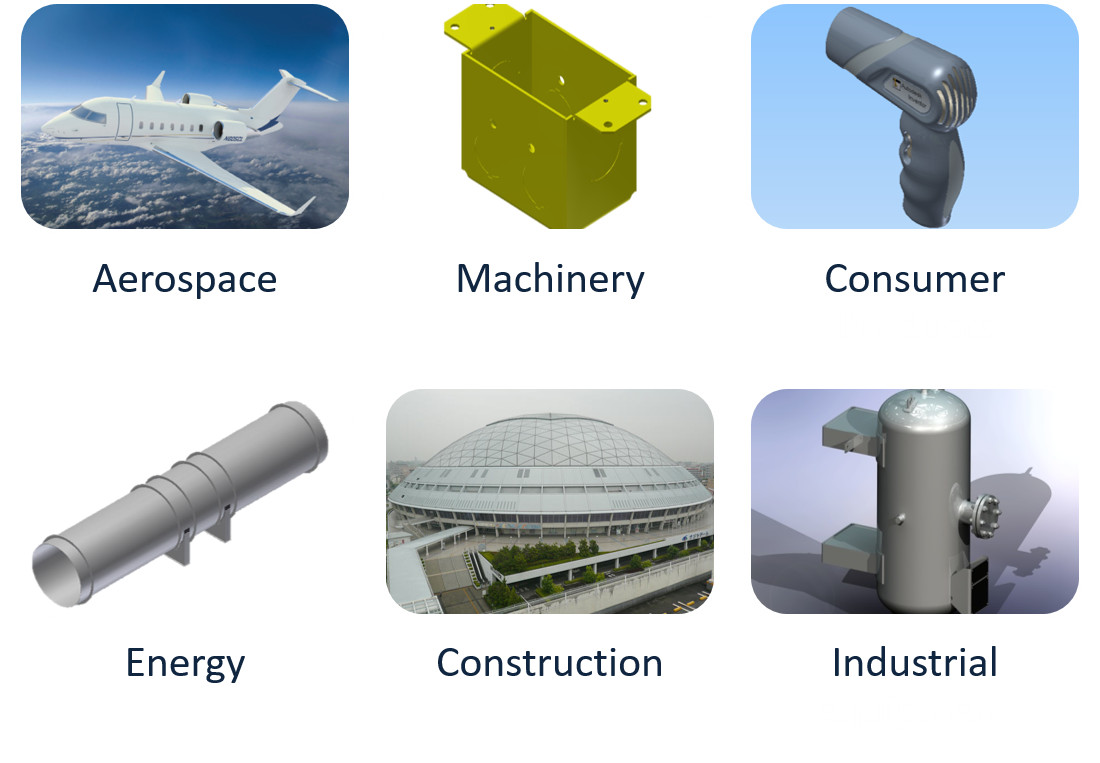
\includegraphics[width=0.9\linewidth,keepaspectratio]{midcurve1}
\end{center}
\end{frame}


%%%%%%%%%%%%%%%%%%%%%%%%%%%%%%%%%%%%%%%%%%%%%%%%%%%%%%%%%%%
\begin{frame}[fragile]\frametitle{Can we use shapes directly?}
	\begin{itemize}
	\item CAD : Designing Shapes
	\item CAE : Engineering Analysis
	\item CAD$\rightarrow$CAE: Simplification for quicker results.
	\end{itemize}

\begin{center}
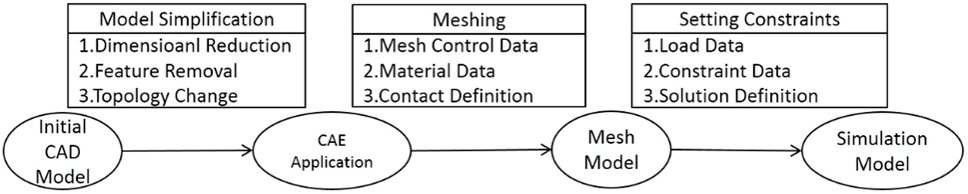
\includegraphics[width=0.9\linewidth,keepaspectratio]{midcurve2}
\end{center}

\end{frame}

%%%%%%%%%%%%%%%%%%%%%%%%%%%%%%%%%%%%%%%%%%%%%%%%%%%%%%%%%%%%%%%%%%%%%%%%%%%%%%%%%%
\begin{frame}[fragile]\frametitle{CAD-CAE}
\begin{center}
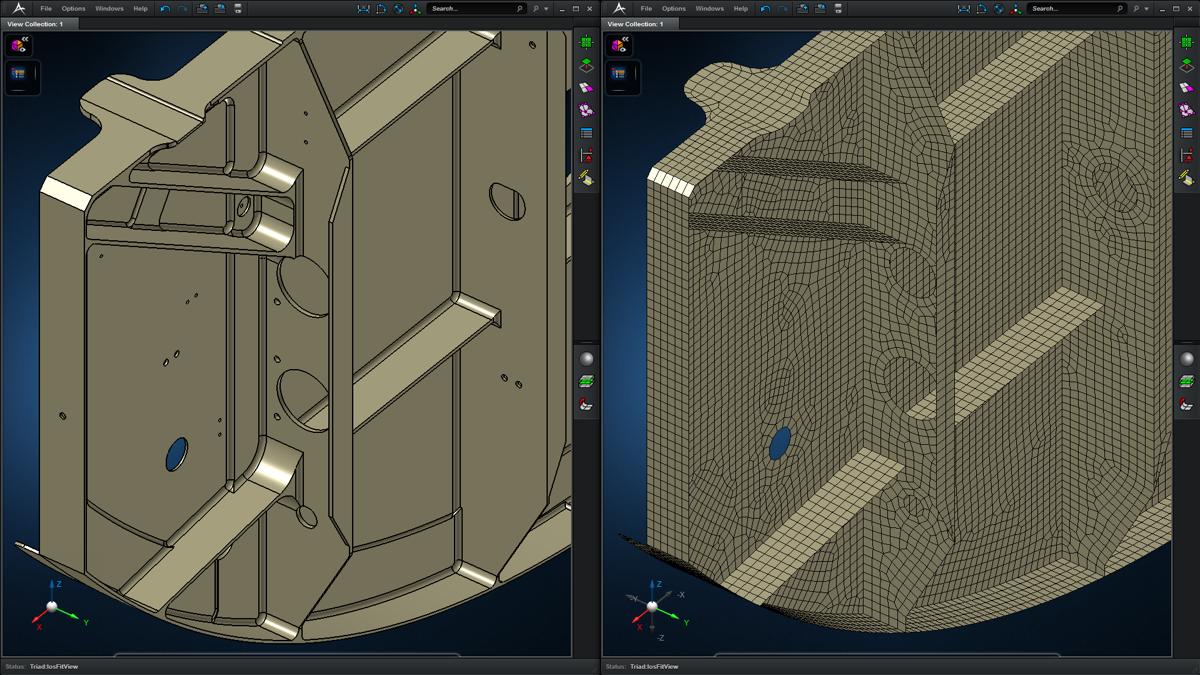
\includegraphics[width=0.9\linewidth,keepaspectratio]{midcurve3}
\end{center}
\end{frame}

%%%%%%%%%%%%%%%%%%%%%%%%%%%%%%%%%%%%%%%%%%%%%%%%%%%%%%%%%%%%%%%%%%%%%%%%%%%%%%%%%%
\begin{frame}[fragile]\frametitle{For Shapes like Sheet Metal \ldots}
\begin{center}
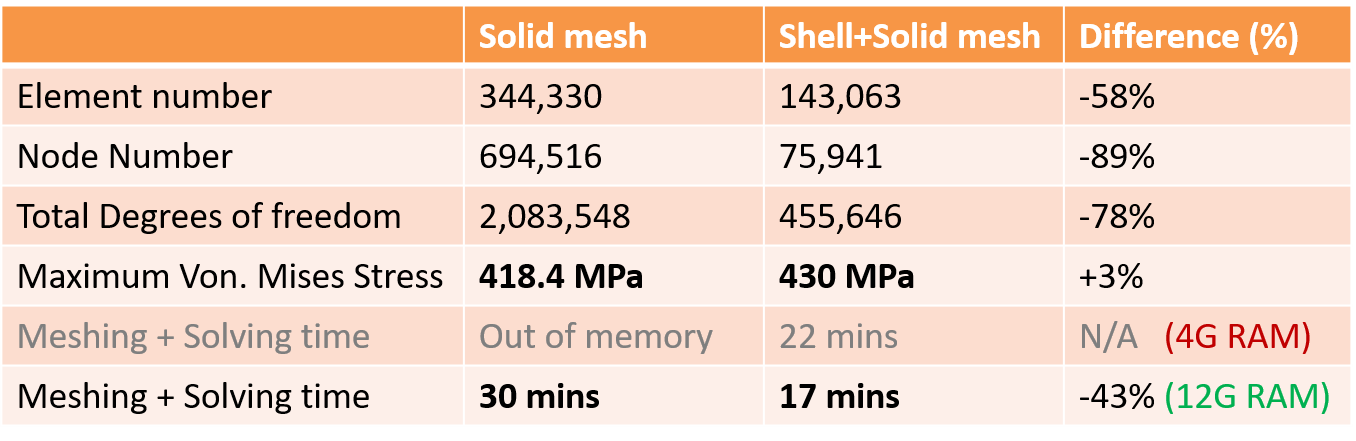
\includegraphics[width=0.9\linewidth,keepaspectratio]{midcurve4}
\end{center}
Half the computation time, but similar accuracy
\end{frame}

%%%%%%%%%%%%%%%%%%%%%%%%%%%%%%%%%%%%%%%%%%%%%%%%%%%%%%%%%%%%%%%%%%%%%%%%%%%%%%%%%%
\begin{frame}[fragile]\frametitle{Midsurface is?}
\begin{center}
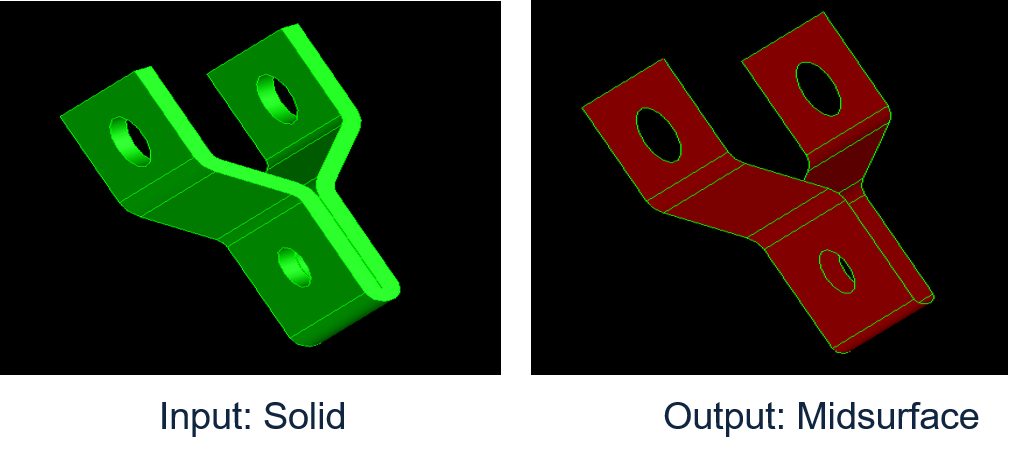
\includegraphics[width=0.9\linewidth,keepaspectratio]{midcurve5}
\end{center}
	\begin{itemize}
	\item Widely used for CAE of Thin-Walled parts
	\item Computation is challenging and still unsolved
	\end{itemize}
	
\end{frame}

%%%%%%%%%%%%%%%%%%%%%%%%%%%%%%%%%%%%%%%%%%%%%%%%%%%%%%%%%%%%%%%%%%%%%%%%%%%%%%%%%%
\begin{frame}[fragile]\frametitle{Getting Midsurface}

	\begin{itemize}
	\item Going on for decades \ldots
	\item Manually by offsetting and stitching, initially
	\item Many CAD-CAE packages give automatic option, but \ldots
	\end{itemize}
\begin{center}
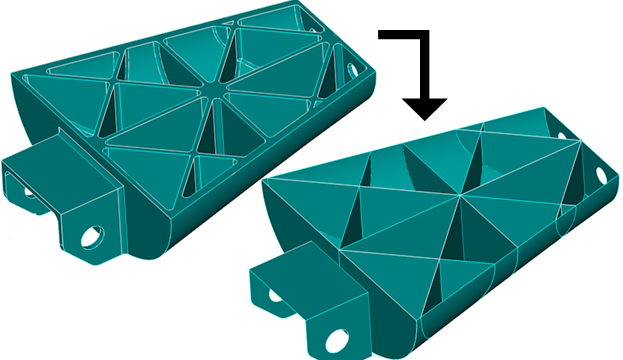
\includegraphics[width=0.6\linewidth,keepaspectratio]{midcurve6}
\end{center}	
\end{frame}

%%%%%%%%%%%%%%%%%%%%%%%%%%%%%%%%%%%%%%%%%%%%%%%%%%%%%%%%%%%%%%%%%%%%%%%%%%%%%%%%%%
\begin{frame}[fragile]\frametitle{Look at the output}
\begin{center}
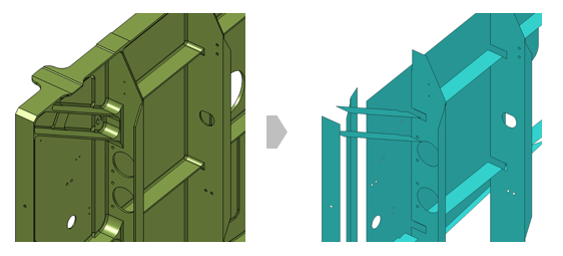
\includegraphics[width=0.9\linewidth,keepaspectratio]{midcurve7}
\end{center}	
\end{frame}

%%%%%%%%%%%%%%%%%%%%%%%%%%%%%%%%%%%%%%%%%%%%%%%%%%%%%%%%%%%%%%%%%%%%%%%%%%%%%%%%%%
\begin{frame}[fragile]\frametitle{Can't tolerate gaps}

	\begin{itemize}
	\item We have thickness sampling, 
	\item To recreate-represent the original shape
	\item Input and output difference not desirable
	\end{itemize}
\end{frame}

%%%%%%%%%%%%%%%%%%%%%%%%%%%%%%%%%%%%%%%%%%%%%%%%%%%%%%%%%%%%%%%%%%%%%%%%%%%%%%%%%%
\begin{frame}[fragile]\frametitle{For a simple model like}
\begin{center}
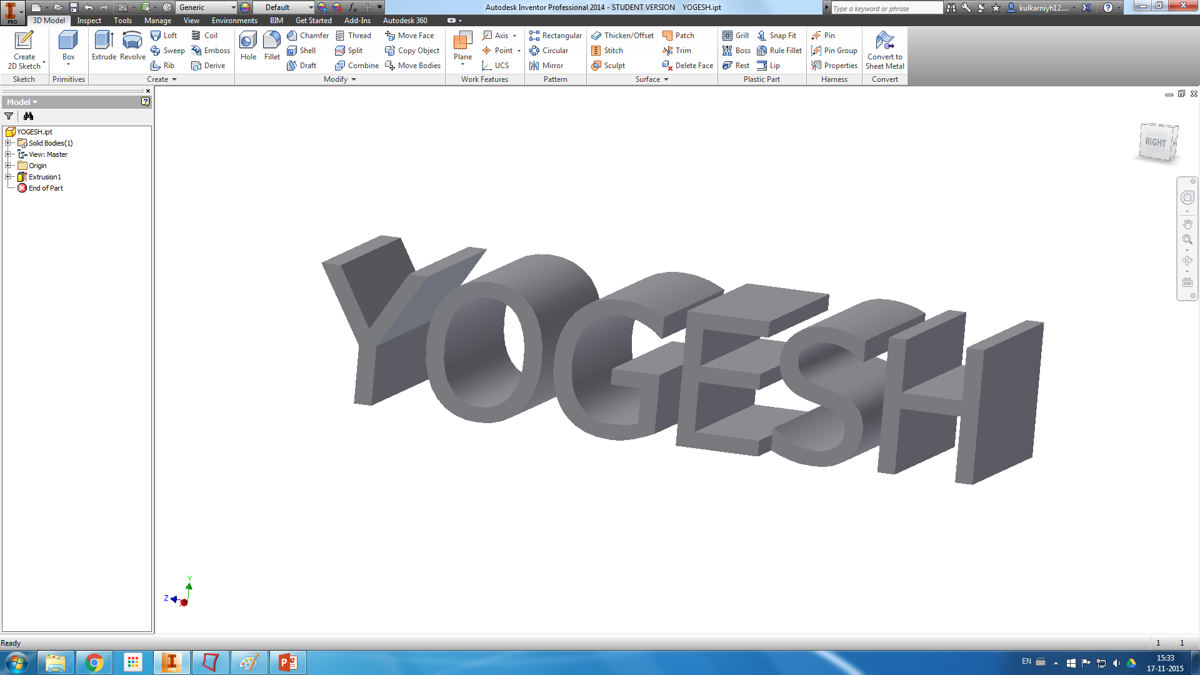
\includegraphics[width=0.9\linewidth,keepaspectratio]{midcurve8}
\end{center}	
\end{frame}

%%%%%%%%%%%%%%%%%%%%%%%%%%%%%%%%%%%%%%%%%%%%%%%%%%%%%%%%%%%%%%%%%%%%%%%%%%%%%%%%%%
\begin{frame}[fragile]\frametitle{You get}
\begin{center}
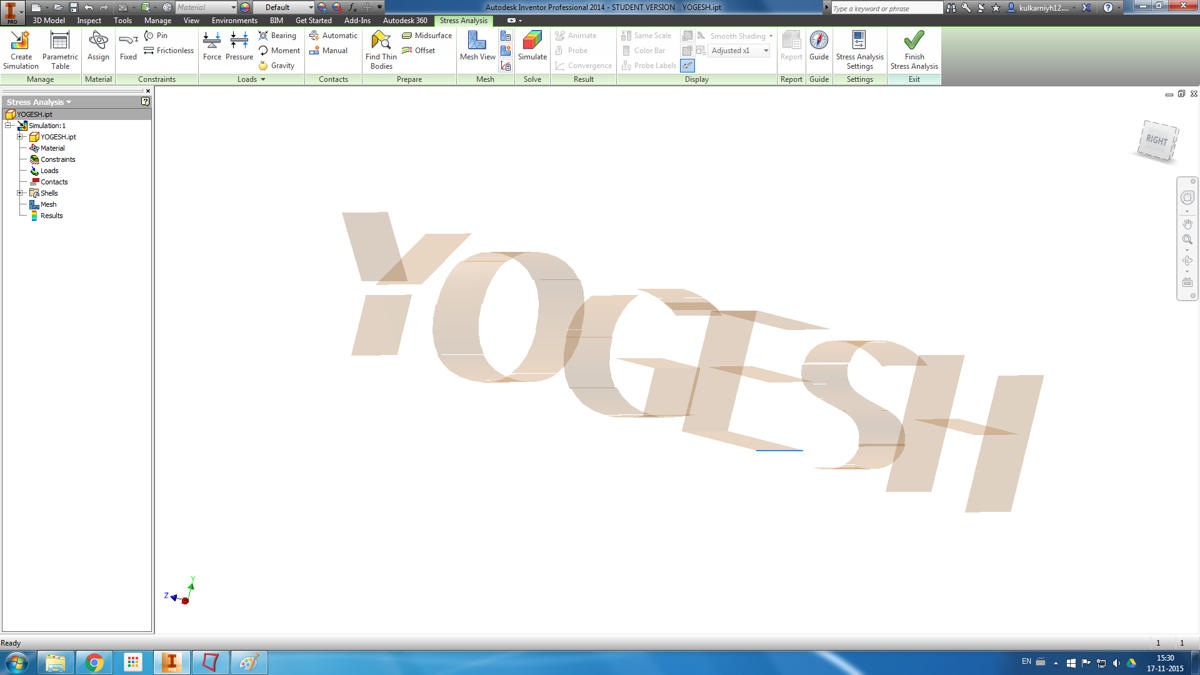
\includegraphics[width=0.9\linewidth,keepaspectratio]{midcurve9}
\end{center}	
\end{frame}

%%%%%%%%%%%%%%%%%%%%%%%%%%%%%%%%%%%%%%%%%%%%%%%%%%%%%%%%%%%%%%%%%%%%%%%%%%%%%%%%%%
\begin{frame}[fragile]\frametitle{For a far simpler shape}
\begin{center}
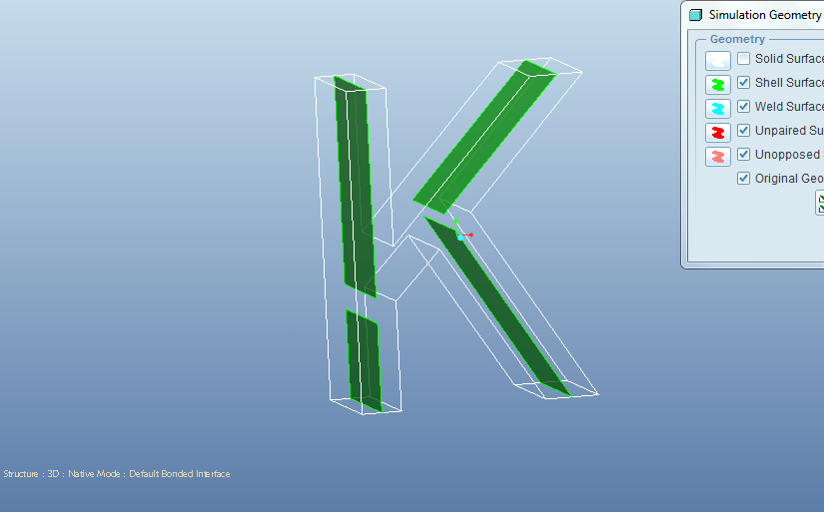
\includegraphics[width=0.9\linewidth,keepaspectratio]{midcurve10}
\end{center}	
\end{frame}

%%%%%%%%%%%%%%%%%%%%%%%%%%%%%%%%%%%%%%%%%%%%%%%%%%%%%%%%%%%%%%%%%%%%%%%%%%%%%%%%%%
\begin{frame}[fragile]\frametitle{Current Quality}
\begin{center}
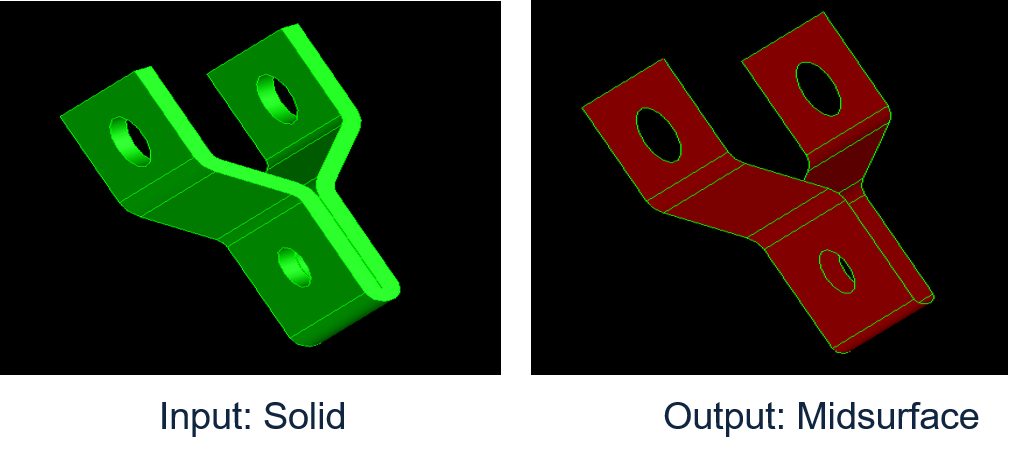
\includegraphics[width=0.6\linewidth,keepaspectratio]{midcurve5}
\end{center}
	\begin{itemize}
	\item Errors take weeks to correct for complex parts.
	\item But still preferred, due to vast savings time
	\item From Days to hours \ldots
	\end{itemize}
	
\end{frame}

%%%%%%%%%%%%%%%%%%%%%%%%%%%%%%%%%%%%%%%%%%%%%%%%%%%%%%%%%%%%%%%%%%%%%%%%%%%%%%%%%%
\begin{frame}[fragile]\frametitle{Midsurface Computation}

	\begin{itemize}
	\item Midsurface of a Patch is Midcurve of its profile extruded.
	\item So, it boils down to computing 1D midcurve of a 2D profile
	\end{itemize}
\begin{center}
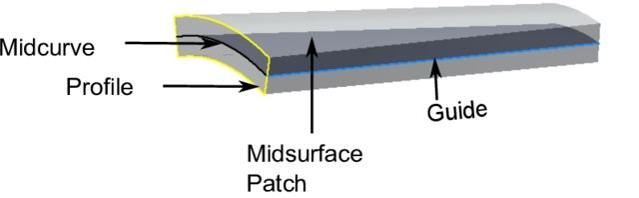
\includegraphics[width=0.6\linewidth,keepaspectratio]{midcurve12}
\end{center}	
\end{frame}

%%%%%%%%%%%%%%%%%%%%%%%%%%%%%%%%%%%%%%%%%%%%%%%%%%%%%%%%%%%%%%%%%%%%%%%%%%%%%%%%%%
\begin{frame}[fragile]\frametitle{What is a Midcurve?}

	\begin{itemize}
	\item Midsurface : From 3D thin Solid to 2D Surface
	\item Midcurve : From 2D Profile to 1D Curve
	\end{itemize}
\begin{center}
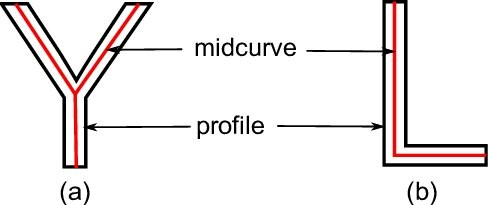
\includegraphics[width=0.6\linewidth,keepaspectratio]{midcurve13}
\end{center}	
\end{frame}